\section{Methodology} \label{isect2}
\subsection{Existing approaches and related literature}

The measurement of the gender-based wage gap can be traced back to the seminal works of~\citet{Oaxaca1973} and~\citet{Blinder1973}, wherein the mean wage gap was decomposed into composition and structure effects. This methodological development spurred a substantial body of research over the past half century, aimed at refining and extending the Oaxaca-Blinder decomposition beyond the single-point estimate of the wage distribution~\citep{Fortin2011}. Methodological extensions to the entirety of the wage distribution enable the identification of gender gaps specific to particular wage groups, developing a deeper understanding of differences both between and within groups~\citep{Machado2005}. Recent applications of distributional decomposition include study of wage gap~\citep{Maasoumi2019}, educational achievements~\citep{Le2018},  and regional inequalities~\citep{Jemmali2023}, among others.\par

A major hurdle in distributional decomposition is constructing a counterfactual distribution, which cannot be directly observed. As a result, in decomposition literature, a significant amount of effort has been devoted to developing methods for constructing counterfactuals.~\citet{DiNardo1996} use kernel density reweighing, while~\citet{Firpo2009} utilise a recentered influence function.~\citet{Machado2005} deploy quantile regression to estimate the inverse conditional distribution function. In contrast,~\citet{Chernozhukov2013} tackle the problem by directly estimating the conditional distributional regression model using quantile regression.\par

In addition to going beyond means, addressing the selection concern has been an important issue in studying gender wage differentials. Four major strategies have been developed in the literature: (a) imputation, (b) identification at infinity, (c) parametric modeling of selection, and (d) the bounding approach~\citep{Machado2017}. The imputation method involves utilizing observed covariates and economic model-based restrictions to impute values for the missing part of the data, i.e., those who do not participate in the work. In a recent application,~\citet{Blau2021}, searched backward and forward in the panel data to find proxy for missing wages by the wage observation in the nearest wave. In contrast, identification at infinity circumvents the selection issue by limiting itself to a much smaller segment of the labour force where participation rates are very high and selection is considered negligible~\citep{Machado2017,Mulligan2008,Heckman1990}. The parametric approach to selection correction is bolder: it aims to explicitly model the selection process, either at the mean~\citep{Newey2009, Heckman1979, Heckman1974} or at quantiles~\citep{Buchinsky1998}. In these models, the outcome and the latent selection equations exhibit linearity with respect to covariates, and error terms are assumed to be independent of covariates, conditional on the selection probability. In comparison, the bounding approach has a lesser ambition as it only seeks to tighten the worst-case scenario bounds on the gender wage gap via restrictions motivated by economic theory~\citep{Blundell2007}. However, as these restrictions -- availability of an instrument to tighten the bound, pre-suppositions on the selection’s sign, or both -- being weaker than parametric modeling produce wider bounds on estimates.\par

In the spirit of ~\citet{Buchinsky1998}, we correct for selection vi\'{a} a parametric approach in the quantile framework. However, we use a copula-based technique~\citep{Arellano2017} to model the joint distribution of error terms in outcome and selection models. This approach overcomes~\citet{Huber2015}'s critique concerning the conditional independence assumption in sample selection models, particularly its implication of identical slopes across all quantile regressions. With additional restrictions compared to the bounding approach, our methodology provides tighter bounds and greater flexibility in capturing the direction of sample selection from the observed data, rather than relying solely on theoretical priors.\par

\subsection{Selection in  a distributional decomposition} \label{subsec:decomposition}
We use a standard employment and wage generating model with 
\begin{linenomath*}\begin{align}
	Y^{*} &= q(U, X),\\
	E &= \mathbbm{1} \{V\leq p(Z)\},\\
	Y &= Y^{*} \text{~if~}E = 1,
\end{align} \end{linenomath*} 
where the latent wage $Y^{*}$ is a function of wage determining observables $X$ and unobservables $U$. The $V$ is the difference in unobservables of the reservation and market wage equations, which, jointly with $Z = (B,X)$, defines the employment status $E$. Since we can only observe wage $Y$ of  those employed, we are left with a sample selection bias dictated by the dependence structure between two sets of unobservables, $U$ and $V$. Furthermore, the $Z$ strictly contains $X$, and the instrument $B$ influences employment status but not the wage.\par

Given the availability of: an exclusion restriction $((U,V) {\perp\!\!\!\perp} Z| X )$; continuous joint distribution of $(U,V)$, defined as $C_{x}(u,v)$, strictly increasing in $u$; a continuous outcome such that $\tau\mapsto q(\tau, x)$ is strictly increasing and continuous in $\tau$; and a  propensity score, $p(Z)\equiv \Pr(E=1|Z)$, which is always greater than zero, ~\citet{Arellano2017} demonstrate that the observed rank for the $\tau^{th}$ quantile, $q(\tau, x)$, is no longer the $\tau$ in the selected sample, i.e.,
\begin{linenomath*}\begin{align}
	\begin{split}		
		\Pr(Y^{*}\leq q(\tau, x)|E=1, Z=z) = Pr(U\leq \tau| V\leq p(z), Z=z)
		&=G_{x}(\tau, p(z)) \\
		&\equiv C_{x}(\tau, p)/p.
	\end{split}
\end{align}\end{linenomath*}
Instead, the conditional copula $G_{x}$ maps ranks $\tau$ in the distribution of $Y^{*}$ conditional on $X=x$ to ranks $G_{x}(\tau, p(z))$ in the distribution of $Y$ conditional on $Z=z$. Thus,  for all $\tau \in (0,1)$, the conditional $\tau$-quantile of $Y^{*}$ coincides with the conditional $G_{x}(\tau, p(z))$-quantile of $Y$ given $E=1$. As a result, knowing $G_{x}$ map from latent to observed ranks mean we can recover $q(\tau, x)$ as a quantile of observed outcomes by shifting the percentile ranks. \par

We work with linear quantile functions, which are selection corrected in three steps: first, propensity score $\hat{p}$ is computed using a probit model; second, copula parameter $\hat{\rho}$ is estimated; and third, given $\hat{p}$ and $\hat{\rho}$, $\tau$th quantile regression coefficient $\hat{\beta}_{\tau}$ is computed. The Frank copula is used to model the dependence structure between $U$ and $V$. The choice of the Frank copula is motivated by its simplicity, as it relies on a single parameter $\rho$; moreover, the Frank copula demonstrates considerable flexibility, allowing for a wide range of data-driven dependencies, including negative ones. In addition, $\rho$ has a useful interpretation; a negative $\rho$ implies positive selection into employment, and vice-versa.  Additionally, we examine the robustness of the results on copula choice and provide Gaussian copula-based estimates.\par 

Using the law of iterated probabilities, we can expand the wage cumulative distribution function conditional on gender $F_{Y_{g}|D_{g}}$ to an integral of conditional outcome over the observed characteristics as
\begin{linenomath*}\begin{align}
	F_{Y_{g}|D_{g}}(y) = \int F_{Y_{g}|X,D_{g}}(y|X=x)\cdot dF_{X|D_{g}}(x), \hspace{2em} g\in (m,f). 
\end{align}\end{linenomath*}
To construct counterfactuals, e.g., what would be women's wages if they were paid like men, we can either manipulate $F_{X}$, as in~\citet{DiNardo1996}, or $F_{Y|X}$ as in~\citet{Chernozhukov2013}. The former approach uses re-weighting by propensity scores, which is not easily extended to address selection~\citep{Maasoumi2017}, while the latter estimates conditional distribution of the outcome employing conditional quantile regression. We follow~\citet{Chernozhukov2013} and swap selection-corrected conditional quantile regression coefficients across groups to construct a counterfactual scenario of females' returns being like men's as 
\begin{linenomath*}\begin{align}
	F_{Y_{m}^{C}:X=X|D_{f}}(y) = \int F_{Y_{m}|X,D_{m}}(y|X=x)\cdot dF_{X|D_{f}}(x).
\end{align}\end{linenomath*}

With the counterfactual in hand, we can apportion the total difference between male and female wage distribution $(TE \equiv F_{Y_{f}:X=X|D_{f}}  - F_{Y_{m}:X=X|D_{m}})$
into differences due to differing returns to labour market characteristics (structural effect or SE) and differential distribution of those characteristics (composition effect or CE), i.e.,
\begin{linenomath*}\begin{align}
	\begin{split}		
		TE &= \left[F_{Y_{f}:X=X|D_{f}} - F_{Y_{m}^{C}:X=X|D_{f}}\right] + \left[F_{Y_{m}^{C}:X=X|D_{f}} - F_{Y_{m}:X=X|D_{m}}\right]\\
		&= SE + CE. \label{eq:TEdefn}
	\end{split}
\end{align}\end{linenomath*}

We assume men to be the baseline and did not model men’s selection into the workforce. The lack of a suitable instrument for men’s workforce participation contributes to this methodological decision. As a result, the selection-adjusted and -unadjusted results differ in SE and total effect (TE), but not in CE. The practical implementation of the wage equation includes years of schooling, experience, experience squared, caste group, marital status, total hours spent on household chores, buildup density in the district, and average district level out-migration. These variables are similar to the human capital specifications of~\citet{Blau2017} and the implementation found in~\citet{Maasoumi2019}. Details on the variable construction are available in the annex.\par
                                   
\subsection{IV and the exclusion restriction}
In the literature, spousal income and number of children are two popular instrumental variables (IV) used for women’s selection into the labour force. The pioneering work of~\citet{Heckman1974} uses number of children in a shadow price function, whereas others have used it as an instrument~\citep{Mulligan2008, Maasoumi2019, Heckman1980, chang2011labor, Lee2009}. The underlying argument of the IV is that the increased cost of childrearing will deter women from participating in the labour force. The strength of this exclusionary assumption depends on socioeconomic norms, which can vary widely across developed and developing economies. In Nepal, families are multi-generational, and childrearing is often shared with grandparents. Additionally, in the labour force surveys, we can observe that most of the women’s labour participation is after the average age of the first childbirth (see figure \ref{fig:ageWiseFemaleParticipation}), which is approximately 20 years~\citep{DHS2016}. Use of the second IV (non-wife spousal income) -- which is used in~\citet{schafgans1998ethnic, Martins2001} -- requires a richer dataset than that available to us.\par

\begin{figure}[h] 
	\centering
	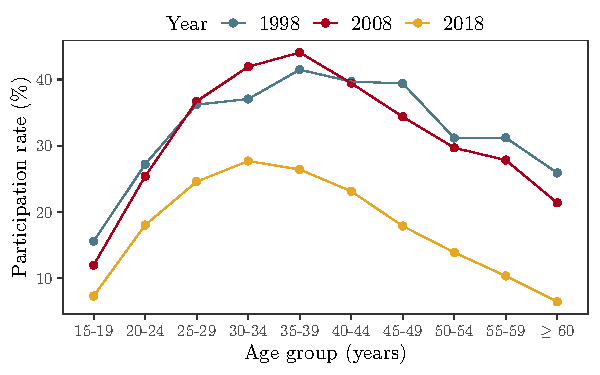
\includegraphics{./figure/AgeWise_femalParticipation_NLFS_all}
	\caption{Female labor force participation with age group}
	\label{fig:ageWiseFemaleParticipation}
\end{figure}  

In this context, we use the ratio of number of other wage earners to total working-age population as an IV to determine female labour force participation. The key assumption is that it is plausible for women to specialise in home production and stay out of the labour market if other family members are already earning. In addition, the use of share instead of directly using non-wife wages avoids the problem of using spousal income, as high-wage earners marry similarly-earning partners. A similar exclusion restriction strategy in conjunction with other instruments is implemented by~\citet{BenYahmed2018}. Additionally, we utilise the test developed by~\citet{Huber2014} to examine the validity of the instrument; they show that assumptions of exclusion restriction and positive monotonicity of selection instrument in the standard employment and wage-generating model entail following two inequality constraints
\begin{linenomath*}\begin{align}
		\mathbb{E}(Y|B=1, E=1, Y\leq y_{\text{q}})  \leq \mathbb{E}(Y|B=0, E=1) \leq  \mathbb{E}(Y|B=1, E=1, Y\geq y_{1-\text{q}}),
\end{align}\end{linenomath*} 
 where  $\text{q}$ is the proportion of always-selected in the mixed population, and $ y_{\text{q}}$ is the $\text{q}$-th conditional quantile in the conditional outcome distribution given $B =1$ and $E = 1$. These twin inequalities can be jointly tested using following null hypothesis: 
\begin{linenomath*}\begin{align}
		H_{0}:  \begin{pmatrix}
			\mathbb{E}(Y|B=1, E=1, Y\leq y_{\text{q}}) - \mathbb{E}(Y|B=0, E=1)  \\
			\mathbb{E}(Y|B=0, E=1) - \mathbb{E}(Y|B=1, E=1, Y\geq y_{1-\text{q}})  
		\end{pmatrix} \leq \begin{pmatrix} 0\\0\end{pmatrix}.
\end{align}\end{linenomath*}  
We discretise the instrument with presence of any other wage earner in the household as one and zero otherwise, and we test the joint hypothesis using mean and probability constraints. We fail to reject the proposed IV in all of our datasets, even when considering all types of data partitions. In contrast, the number of children in the family as an IV either fails to converge or is rejected by the test in most of the datasets. The test results are available in the annex.\par  

\subsection{Household dynamics in female participation}

We check for the role of household dynamics in women’s labour market outcomes vis-\'{a}-vis men in two ways. First, we look into the effect of earning potentiality on job participation; second, we examine the gender gap in time allocated for home production. For the first, we explore how differential earning potential changes the probability of women’s engagement in employment using a census dataset. We use the male–female gap in average years of schooling as a proxy for earning potential. The basic regression is a logit model for the probability that woman $f$ in household $h$ participates in employment as an employee 
\begin{linenomath*}\begin{align}
	P(\text{Employee}_{f, h}) = GAP_{h}\beta+ X_{f}\gamma+ Z_{h}\delta+ \psi_{u} + \pi_{d} + \epsilon_{f,h}, \label{eqn:earningPotRegEqn}
	\end{align}\end{linenomath*} 
where $GAP_{h}$ is male minus female average years of schooling in household $h$, $X_{f}$ is a vector of the individual characteristics of woman $f$, $Z_{h}$ is a vector of household characteristics, $\psi_{u}$ is urban dummy, $\pi_{d}$ are district dummies, and $\epsilon_{f,h}$ is the stochastic error term.\par

This $GAP_{h}$ is a rough measure, as it compares all working-age female household members with male members. For a sharper measurement of earning potential differences, we look into spousal pairs, replacing $GAP_{h}$ in equation (\ref{eqn:earningPotRegEqn}) with $GAP_{f}$, which is the gap in years of schooling between a woman and her husband. We extract two types of spousal pairs from the census: the first type is a son and daughter-in-law pair, and the second type is household head and their spouse. These two types of spousal gaps allow us to examine differences caused by the degree of responsibility for home production. For robustness of the specifications, we also check the probit versions of the discussed models. Furthermore, we contrast the results of the probability of a woman being employed against female engagement in own-account work.\par 

For the second, we run a baseline OLS model of time spent on doing household chores by individual $i$ of household $h$ as
\begin{linenomath*}\begin{align}
	TimeSpent_{i} = F\beta_{1} + E\beta_{2} + (F\times E)\beta_{3} + X_{i}\gamma+ Z_{h}\delta+ \psi_{u} + \epsilon_{i,h},
	\end{align}\end{linenomath*} 
where $F$ is a female dummy, $E$ is an employed dummy, $F\times E$ is an interaction term, $X_{i}$ is a vector of individual characteristics, $Z_{h}$ is a vector of household characteristics, $\psi_{u}$ is urban dummy, and $\epsilon_{i,h}$ is the stochastic error term. Years of schooling, age, and age squared are included in $X_{i}$, while house ownership, land ownership, household size, and caste group are included in $Z_{h}$.  The time spent doing household chores is defined as total hours spent on home production and running household-related errands. Complete variable descriptions are available in the annex.\par

Coefficients of interest are $\hat{\beta}_{1}, \hat{\beta}_{2}$, and $\hat{\beta}_{3}$; these provide information on gender-wise differential time allocation. For robustness of coefficients, we use two strategies. First, we construct variables with the same definitions from the living standard survey (2011) and the labor force surveys (2008, 2018) to conduct baseline regressions. Second, we remove variation associated with personal and household characteristics using statistical matching, followed by regression. We use the Mahalanobis distance matching, using a generalized full-matching approach that assigns every unit to a subclass and minimises the largest within-subclass distances in the matched sample~\citep{Savje2021}. Data balance, both before and after matching, is reported in annex figure A7.\par 

\subsection{Data sources}

We compute wage gap through three rounds of the nationally representative Nepal Labour Force Survey (NLFS), produced by the National Statistics Office (NSO) (formerly known as the Central Bureau of Statistics (CBS)) in 1998, 2008, and 2018. These multistage stratified random sampling surveys consider geographical domain, urban–rural heterogeneity, and seasonal variation, followed by probable oversampling adjustments. The first round interviewed 14,400 households, and the subsequent rounds interviewed 16,000 and 18,000 households; this resulted in working age (15-65 years) samples of 38,535, 44,734, and 47,905 individuals, respectively. These surveys provide information on cash earnings, from which we extracted employed samples of 6,477 (76\% men and 24\% women), 7,565 (74\% men and 26\% women), and 7,838 (76\% men and 24\% women) people across all rounds. In addition to wages, the surveys report individual and household characteristics, including demographics, skills acquisition, and job market attributes.\par

For the effects of earning potentiality on female labour market participation, we use the Housing and Population Census 2011 of Nepal, also conducted by the NSO. For this analysis, we include all individuals of working age. The census surveyed a total of 5,427,302 households, of which the available micro-data randomly sampled approximately 15.5\% of the total households to get the sample of 841,565 households. Additionally, we extract time use from the third round of the Nepal Living Standard Survey (NLSS III) 2011. It was also conducted by NSO using two stage stratified random sampling with a population frame of the 2011 census. Six thousand households were interviewed across Nepal, leading to a sample size of 18,260 individuals, with 8,074 men and 10,186 women in working age.\par  

 
                            
